\chapter{Abbildungen}
Alle Abbildungen und Tabellen sind laut Richtlinien fortlaufend mit Nummern zu versehen. Diese Aufgabe übernimmt \LaTeX{} für dich. Jedoch solltest du den Text unter dem Bild (Legende) auf das jeweilige Bild anpassen. Hast du das Bild irgendwo entnommen, dann muss der Quellenverweis auch direkt in der Legende mit eingebaut sein.

Im Text selbst solltest du auf die Abbildung verweisen. Neben dem reinen verweisen, solltest du dich auch damit auseinandersetzen. Beschreibe die Grafik, hebe die Relevanz einzelner Teile hervor oder nenne andere wichtige Informationen im Text davor oder danach.

\section{Tabellen}
Die Legende steht bei den Tabellen darüber, während diese bei anderen Grafiken darunter ihren Platz einnimmt.

\begin{table}[ht]
	\centering
	\caption{Eine dreispaltige Tabelle}
	\begin{tabular}{lll}
		\toprule
		\textbf{linke Spalte} & \textbf{mittlere Spalte} & \textbf{rechte Spalte} \\
		\midrule
		A & \makecell{Dies ist ein \\ Umbruch} & C \\
		! & 2 & 3 \\
		a & b & c \\
		i & ii & iii \\
		\bottomrule
	\end{tabular}
	\label{tabelle:Einfache3Spalten}
\end{table}

Bitte beachte auch, dass \LaTeX{} deine Tabellen an eine andere Position verschiebt, wenn diese dort besser aussehen. Vermeide deshalb Textpassagen wie beispielsweise \enquote{in der nachfolgenden Tabelle/Grafik}, denn es könnte sein, dass die Tabelle vor den Text rutscht. Nutze deshalb immer Verweise wie: \enquote{in der Tabelle \ref{tabelle:Zahlenausrichtung} ist \dots }!

Die Tabelle \ref{tabelle:Zahlenausrichtung} nutzt mehrere Packages. Mithilfe des Befehls \texttt{\textbackslash midrule} aus dem Package \enquote{booktabs} erstellt man eine horizontale Linie, die die vertikalen unterbricht. Diese sorgt für ein schöneres Schriftbild. Möchtest du Zahlen auflisten, so kannst du diese nach dem Dezimalkomma ausrichten. Dies geht mit dem Package \enquote{siunitx}.

Mit dem Befehl \texttt{makecell} kann eine einzelne Zelle in einer Tabelle nach durch einen normalen Umbruch umgebrochen werden.

\begin{table}[ht]
	\centering
	\caption{Zahlenausrichtung}
	\begin{tabular}{c|c|r|r|S[table-format=3.7]}
		% Anstatt \hline können \toprule, \bottomrule und \midrule verwendet werden.
		\toprule
		% Hinweis: \multicolumn wird verwendet, um die eigentliche Anordnung zu umgehen.
		Nr.  & Datum & Euro & USD  & \multicolumn{1}{c@{}}{Zahlen} \\ 
		\midrule 
		1  & 01.06.2017 & $1,00$€  & $1,13\$$  & 11,158   \\
		2  & 02.06.2017 & $2,00$€  & $2,26\$$  & 2,18     \\
		3  & 03.06.2017 & $3,00$€  & $3,39\$$  & 9,15568  \\
		4  & 04.06.2017 & $4,00$€  & $4,52\$$  & 5,868668 \\
		5  & 05.06.2017 & $5,00$€  & $5,65\$$  & 1,4      \\
		\midrule
		6  & 06.06.2017 & $6,00$€  & $6,78\$$  & 6,58     \\
		7  & 07.06.2017 & $7,00$€  & $7,91\$$  & 7,998    \\
		8  & 08.06.2017 & $8,00$€  & $9,04\$$  & 4,358    \\
		9  & 09.06.2017 & $9,00$€  & $10,17\$$ & 3,5458   \\
		10 & 10.06.2017 & $10,00$€ & $11,30\$$ & 302,8    \\
		\bottomrule
	\end{tabular}
	\label{tabelle:Zahlenausrichtung}
\end{table}

Die Tabelle \ref{tabelle:Zellenverbindung} zeigt die Möglichkeit, einzelne Zellen miteinander zu verbinden. Mit dem Befehl \texttt{\textbackslash multicolumn \{Anzahl Spalten\}\{Ausrichtung\}\{Inhalt\}} kannst du mehrere Spalten verbinden. Dafür müssen die überschriebenen Spalten entfernt werden, es darf also keinen \enquote{\&}-Trennzeichen dafür geben. Beim Verbinden mehrerer Reihen wird der Befehl \texttt{\textbackslash multirow\{Anzahl Reihen\}\{*\}\{Inhalt\}} verwendet. Hierbei darauf achten, dass die Zellen, die zusammengefasst werden sollen, keinen Inhalt haben, aber vorhanden sind, also einen \enquote{\&}-Trennzeichen besitzen.

\begin{table}[ht]
	\centering
  \caption{Verbinden von Zellen}
	\begin{tabular}{c|c|r}
		\toprule
		Text 1               &      Mittiger Text 2      &   Text 3 \\ \midrule
		\multicolumn{2}{l}{Linksbündig}                  &  1,00 \texteuro \\ \midrule
		   2                 &                           &  2,00 €  \\ \midrule
		   3                 &        03.06.2017         &  3,00 € \\ \midrule
		   4                 &        04.06.2017         &  4,00 € \\ \midrule
		                    \multicolumn{3}{r}{Rechtsbündiger Text} \\ \midrule
		   6                 &        06.06.2017         &  6,00 € \\ \midrule
		   7                 & \multirow{2}{*}{Zusammen} &  7,00 € \\ \cmidrule{1-1} \cmidrule{3-3}
		   8                 &                           &  8,00 € \\ \midrule
		   9                 &        09.06.2017         &  9,00 € \\ \midrule
		  10                 &        10.06.2017         & 10,00 € \\ \bottomrule
	\end{tabular}
	\label{tabelle:Zellenverbindung}
\end{table}

\pagebreak
\section{Grafiken}

\begin{wrapfigure}{l}{0.30\textwidth}
	\centering
	\vspace{-20pt} % Manchmal möchte man den oberen Abstand selbst anpassen
	
\includegraphics[width=0.25\textwidth]{images/desktop-screen.pdf}
	\vspace{-10pt}
	% Das folgende ist ein Trick, um "Abbilgung x.y" in eine
	% eigene Zeile zu packen. Der Text zwischen [ und ] steht
	% im Abbildungsverzeichnis. Der Text darunter wird
	% tatsächlich angezeigt.
	\caption[Wrap Figure mit einer PDF als Grafik]{\unskip}
	Wrap Figure mit einer PDF als Grafik
	\label{fig:wrap-Referenz-auf-Bild}
\end{wrapfigure}
Eine gute Projektarbeit kommt nicht ohne einige Abbildungen in Form von Skizzen, Diagrammen oder  ähnlichem aus.
Am besten ist es, wenn du diese Grafiken selbst als SVG Dateien erstellst und diese in Form eines PDFs einbindest, somit ist die Grafik auch beim Drucken scharf.

Gerade solche Kleinigkeiten zeugen von Professionalität und können auch nochmals einige Punkte für eine gute Note raus holen. Die \texttt{figure} Umgebung eignet sich für das Einbinden von Grafiken, die die volle Seitenbreite ausnutzen. Sie erscheinen nicht im Fließtext.

\begin{figure}
	\begin{subfigure}[c]{0.49\textwidth}
		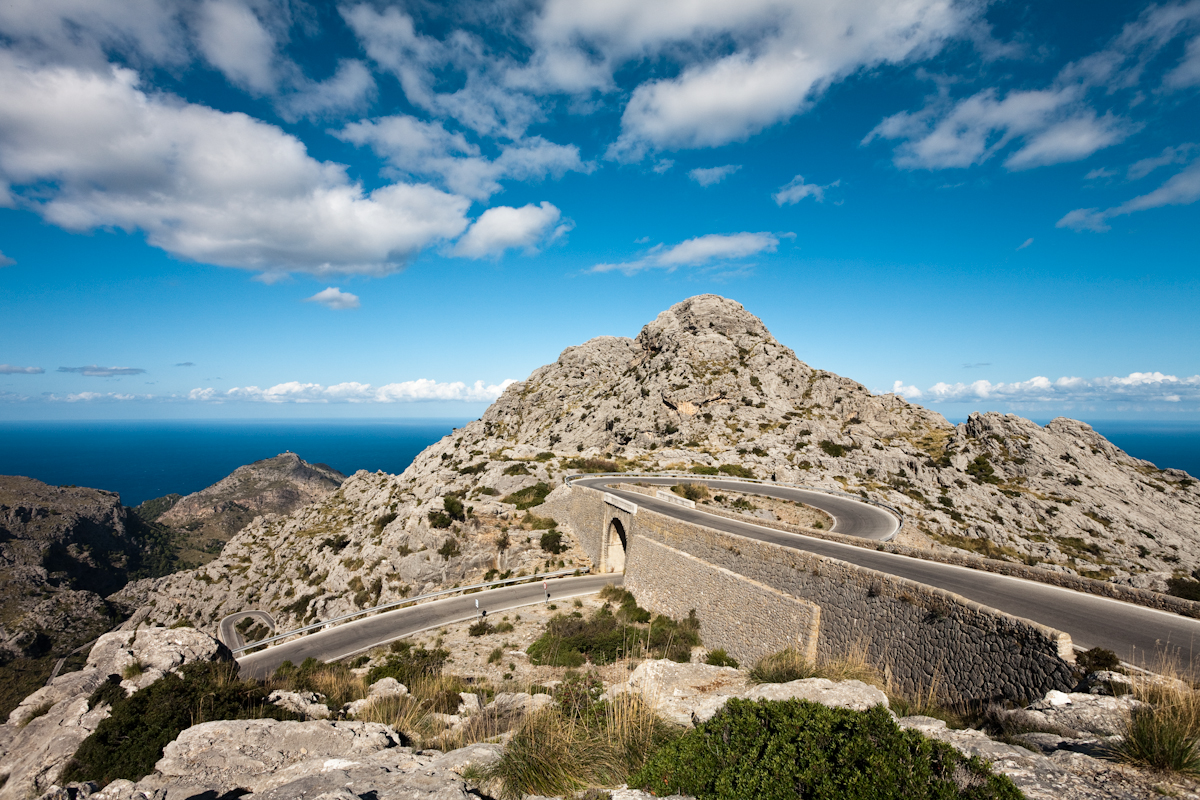
\includegraphics[width=\textwidth]{images/b1.jpg}
		\subcaption{Subfigure Bild Nr. 1}
	\end{subfigure}
	\begin{subfigure}[c]{0.49\textwidth}
		
\includegraphics[width=\textwidth]{images/b2.jpg}
		\subcaption{Subfigure Bild Nr. 2}
	\end{subfigure}
	\caption{Zwei Bilder mit Subfigure nebeneinander}
\end{figure}

Dagegen gibt es die \texttt{wrapfigure} Umgebung, die das Einbinden von Grafiken im Fließtext erlaubt.
Diese Umgebung ist allerdings ab und zu problematisch zu benutzen.
Tipp: Die \texttt{wrapfigure} Umgebung vor dem Absatz platzieren und darauf achten, dass sie nicht in der Nähe eines Seitenumbruchs ist.
Dann erscheint sie rechts oder links des Paragraphen. Mit \texttt{vspace} kann noch der Abstand nach oben und unten angepasst werden, um leeren Platz zu vermeiden.
Siehe auch \url{https://tex.stackexchange.com/questions/56176/handling-of-wrapfig-pictures-in-latex}.

\begin{figure}[ht]
	\centering
	
\includegraphics[width=0.50\textwidth]{images/desktop-screen.pdf} 
	\caption{Desktop Ansicht mit einem Symbol}
	\label{fig:Referenz-auf-Bild}
\end{figure}

Das kostenlose Tool \href{https://inkscape.org/}{\textbf{Inkscape}} hilft dir beim erzeugen dieser SVG Grafiken. Solltest du noch nie damit gearbeitet haben, dann schau dir am besten einige kurze Tutorials an. Im Github Repository unter dem Reiter Wiki findest du eine Kurzanleitung, wie du ein PDF in Inkscape generieren kannst. Solltest du weitere gute kostenlose Software für die Bildbearbeitung in SVG kennen, dann kannst du diese gerne uns per E-Mail mitteilen. Danke!

\section{Diagramme, Mockups, Software Design}

Um Software Designs mit einzubinden eignet sich das Online Tool \textbf{\href{https://www.draw.io/}{DRAW.IO}} sehr gut. Mit diesem Tool lassen sich Diagramme, Mockups, Flow Charts, technische Zeichnungen, Wireframe Skizzen sowie Software Designs zeichnen, welche du ohne Verpixelung im PDF-Format wieder, wie in Abbildung \ref{fig:Diagramm-DrawIo} gezeigt, einbinden kannst.

\begin{figure}[ht]
	\centering
	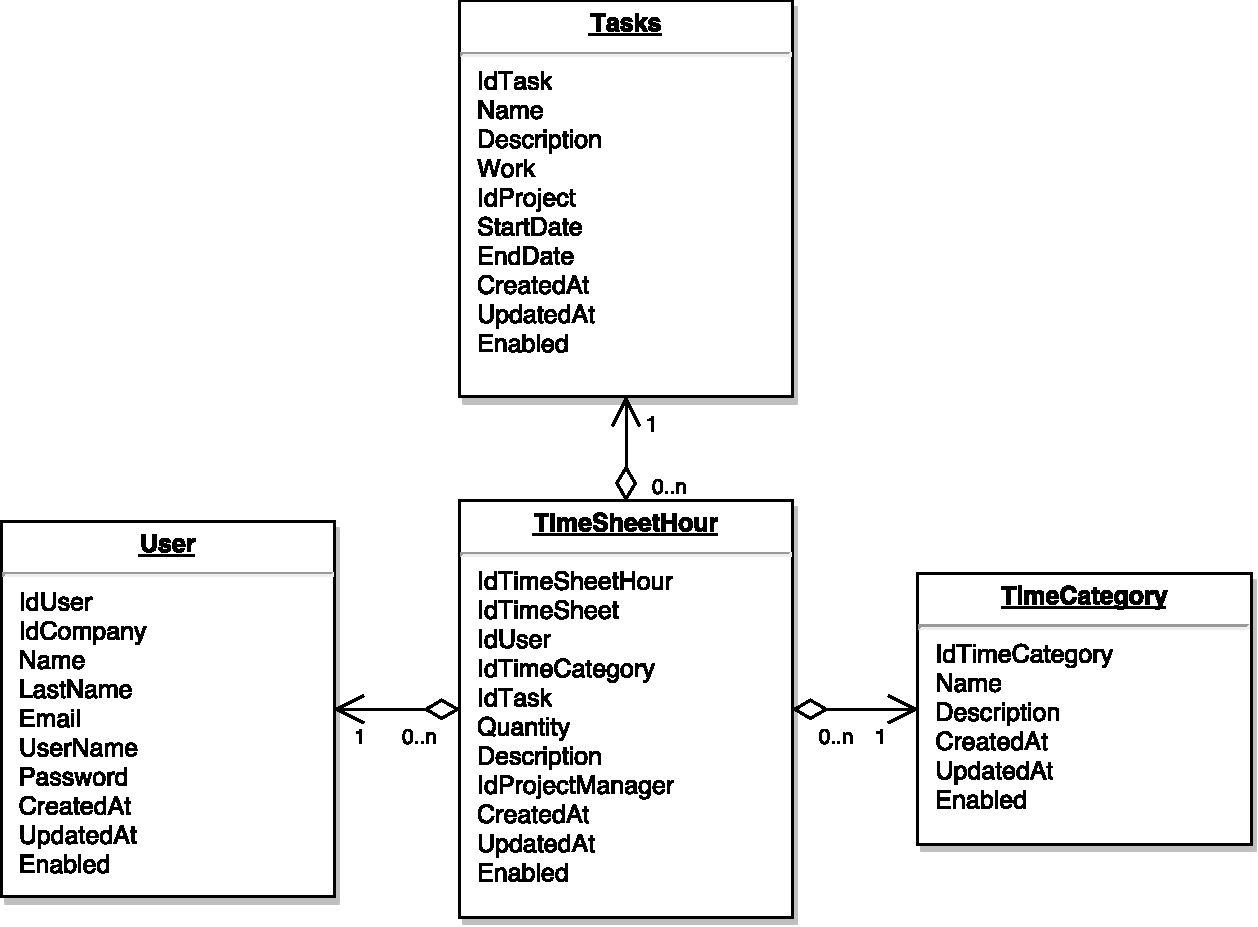
\includegraphics[width=0.8\textwidth]{images/Diagramm.pdf} 
	\caption{Diagramm eines Software Designs}
	\label{fig:Diagramm-DrawIo}
\end{figure}

Ein weiteres kostenloses Tool für die Darstellung von Klassendiagrammen oder auch Sequenzdiagrammen ist \textbf{\href{http://staruml.io/}{StarUML}}. Dieses generiert auch SVG Dateien, welche du mithilfe von Inkscape zu PDF Dateien konvertieren kannst.
